\documentclass{elsarticle}

\usepackage{amsmath,bm}
\usepackage{algorithm}
\usepackage{algpseudocode}
\usepackage{minted}
\usepackage{xcolor}
\usepackage{multirow}
\usepackage{color,soul}
\usepackage{rotating}


\begin{document}

\begin{frontmatter}
\author{Ashwin Srinath \fnref{fn1}}
\author{Daniel Livescu \fnref{fn2}}
\author{Richard S. Miller \fnref{fn1}\corref{cor1}}
 
\fntext[fn1]{Department of Mechanical Engineering, Clemson University, Clemson, SC 29634-0921}
\fntext[fn2]{Los Alamos National Laboratory, Los Alamos, NM 87544, USA}
\cortext[cor1]{Corresponding author. Email address: rm@clemson.edu}

\title{Solution of near-Toeplitz tridiagonal systems on
GPU-accelerated clusters}
  
\begin{abstract}
In this paper, we consider the solution of linear
systems of the form $A\bm{x} = \bm{d}$,
where $A$ is \emph{near-Toeplitz} tridiagonal.
These systems appear in numerical schemes
such as
Alternating Direction Implicit (ADI) methods,
compact finite differences,
and one-dimensional ordinary
and partial differential equations.
We develop a GPU solver that takes advantage
of the known structure of the matrix
to reduce the number of computations
and improve memory access.
Our solver is able to outperform
the NVIDIA CUSPARSE and
multi-core Intel MKL tridiagonal solvers
(on up to 16 cores).
Further, we present a parallelization strategy
for GPU-accelerated clusters,
and show scalability of a compact finite difference applications
for up to 64 GPUs on the Clemson University Palmetto cluster.

\end{abstract}

\end{frontmatter}
  %---------------------------------------------------------------------%
\section{Introduction}
%---------------------------------------------------------------------%

The focus of this paper is the solution of
linear systems of the form $A\bm{x} = \bm{d}$,
where $A$ has the following structure

\begin{equation} \label{eqn:toeplitz-matrix}
A = 
\begin{pmatrix}
     b_1 & c_1  \\
     a_0 & b_0  &  c_0  \\
         & a_0  &  b_0 &  c_0  \\
         &      &  a_0 &  b_0 &  c    \\
         &      &      &      &  \ddots \\
         &      &      &      &     &  \ddots  \\
         &      &      &      &     &  a_n  &  b_n
\end{pmatrix}
\end{equation}
%
where, in general
\begin{align*}
    & a_0 \neq a_n & \\
    & b_1 \neq b_0 \neq b_n &\\
    & c_1 \neq c_0 &
\end{align*}

We refer to matrices with the specific structure of $A$
as \emph{near-Toeplitz tridiagonal matrices},
and the linear system $A\bm{x}=\bm{d}$ as \emph{near-Toeplitz tridiagonal systems}.

Such tridiagonal systems
appear in several numerical schemes
in Computational Fluid Dynamics (CFD)
such as
compact finite differences
\cite{lele1992compact,kennedy1994several},
Alternating Direction Implicit (ADI) methods \cite{1955ADI}, and
numerical solutions of one-dimensional differential equations.
In such applications,
the evaluation of the tridiagonal systems constitutes
a significant portion of the runtime.
Recently, there has been considerable interest in the CFD community
in developing general tridiagonal solvers that
exploit the massive parallelism afforded by
Graphics Processing Units (GPUs)
to speed up the computations
\cite{tutkun2012gpu,esfahanian2014efficient,GoSt11CR}.
The performance of tridiagonal solvers on the GPU
has been shown to depend on several factors,
such as
choice of algorithm and the associated complexity,
thread utilization,
use of the available memory hierarchy,
and synchronization and control costs
\cite{Zhang2010FTS}.
Many approaches described in the literature
seek to make trade-offs between these factors
to arrive at a solver that best fits the requirements.
But to our knowledge,
the algorithms proposed so far
are applicable to general tridiagonal systems,
and make no attempt to take advantage of
the known structure of the tridiagonal matrix.
The contribution of this paper is twofold:
First, we describe the implementation of a GPU solver
for the specific case of \emph{near-Toeplitz} tridiagonal systems
that uses the known structure to reduce
computations and memory accesses.
Second, we describe the implementation for
multi-GPU clusters, i.e., a distributed memory environment,
and apply it to the evaluation of compact finite differences.

This paper is organized as follows:
Section \ref{sec:preliminaries}
reviews the cyclic reduction algorithm,
and its implementation on GPUs.
We also provide some relevant details about GPU architecture here.
Section \ref{sec:proposed-algorithm}
describes our proposed solver for \emph{near-Toeplitz} tridiagonal systems.
Section \ref{sec:gpu-implementation}
discusses the implementation of the algorithm on GPUs.
Section \ref{sec:results-single-gpu}
provides an overview of the performance of our solver,
and compares it with other implementations.
Section \ref{sec-compact-finite-differences}
describes the implementation on multiple GPUs,
and application to the solution of compact finite differences.

%---------------------------------------------------------------------%
\section{Preliminaries} \label{sec:preliminaries}
%---------------------------------------------------------------------%

\subsection{Cyclic reduction} \label{subsec:cyclic-reduction}

\begin{equation} \label{eqn:general-tridiagonal-system}
\begin{pmatrix}
     b_1 & c_1  \\
     a_2 & b_2  &  c_2  \\
         & a_3  &  b_3 &  c_3  \\
         &      &  a_4 &  b_4 &  c_4  \\
         &      &      &      &  \ddots \\
         &      &      &      &     &  \ddots  \\
         &      &      &      &     &  a_n  &  b_n
\end{pmatrix}
\begin{bmatrix}
    x_1 \\
    x_2 \\
    x_3 \\
    x_4 \\
    \vdots \\
    \vdots \\
    x_n
 \end{bmatrix}
=
\begin{bmatrix}
   d_1 \\
   d_2 \\
   d_3 \\
   d_4 \\
   \vdots \\
   \vdots \\
   d_{n}
\end{bmatrix}
\end{equation}

Cyclic reduction is applicable to the solution of
linear systems of the form $A\bm{x} = \bm{d}$,
where $A$ is a tridiagonal matrix with diagonals
$\bm{a}$, $\bm{b}$ and $\bm{c}$
[Eq. (\ref{eqn:general-tridiagonal-system})].
The algorithm consists of two phases:
\emph{forward reduction} and \emph{backward substitution}
(Fig. \ref{fig:cyclic-reduction}).
In the forward reduction phase,
every even-indexed equation $i$
is expressed as a
linear combination of equations $i$, $i-1$ and $i+1$,
yielding a new tridiagonal system of
$n/2$ equations in $n/2$ unknowns
[Eqs. (\ref{eqn:forward-reduction-1}) - (\ref{eqn:forward-reduction-4})].
The process is repeated until a system of
2 equations in 2 unknowns is left.

\begin{align} 
& a^{\prime}_i = -a_{i-1}k_1 \
    \label{eqn:forward-reduction-1}& \\
& b^{\prime}_i = b_i - c_{i-1}k_1 - a_{i+1}k_2 \
    \label{eqn:forward-reduction-2}& \\
& c^{\prime}_i = -c_{i+1}k_2 \
    \label{eqn:forward-reduction-3}& \\
& d^{\prime}_i = d_i - d_{i-1}k_1  - d_{i+1}k_2 \
    \label{eqn:forward-reduction-4}&
\end{align}
%
where,

\begin{align}
& k_1 = \frac{a_i}{b_{i-1}} \label{eqn:k1-update}& \\
& k_2 = \frac{c_i}{b_{i+1}} \label{eqn:k2-update}&
\end{align}

The 2-by-2 system of equations is solved trivially,
yielding $x_n$ and $x_{n/2}$.
In the backward substitution phase,
every odd-indexed unknown $x_i$ is solved for by
substituting the known values of $x_{i-1}$ and $x_{i+1}$
[Eq. (\ref{eqn:backward-substitution})].

\begin{align} \label{eqn:backward-substitution}
x_i = \frac{d^{\prime}_i - a^{\prime}_ix_{i-1} - \
    c^{\prime}_ix_{i+1}}{b^{\prime}_i}
\end{align}
%
For the last index $i=n$,
the forward reduction step is instead:
\begin{align} \label{eqn:forward-reduction-last}
    & a^{\prime}_n = -a_{n-1}k_1 & \\
    & b^{\prime}_n = b_n - c_{n-1}k_1 & \\
    & d^{\prime}_n = d_n - d_{n-1}k_1&
\end{align}
%
And for $i=1$, the backward substitution step is instead:
\begin{align} \label{eqn:backward-substitution-first}
x_1 = \frac{d^{\prime}_1 - c^{\prime}_1x_{2}}{b^{\prime}_1}
\end{align}

\hl{
Thus, cyclic reduction requires \emph{significantly} fewer steps
($2log_2(n) - 1$) compared to Thomas algorithm ($2n$).
Each step in cyclic reduction consists of operations on several indices
that can each be done independently,
suggesting a parallel (multi-threaded) approach.
When solving linear systems with the same matrix but several right hand sides,
a thread-parallel Thomas algorithm in which
each thread solves an independent system may be considered.
Mattor et al. suggest that this may be a more efficient use
of parallelization compared to cyclic reduction,
due to the smaller amount of work required per thread.
However, using cyclic reduction for solving the independent systems
exposes a larger amount of parallelism -
which is important for good performance on GPUs.
When the number of systems to be solved is small
(as is the case in 2-D problems and small 3-D problems),
the thread-parallel Thomas algorithm under-utilizes the GPU.
For larger problems,
successive threads access far-apart memory locations,
leading to poor GPU performance.
Thus, we argue that cyclic reduction is a better fit for
massively parallel architectures such as GPUs.
}

\begin{figure}
\begin{center}
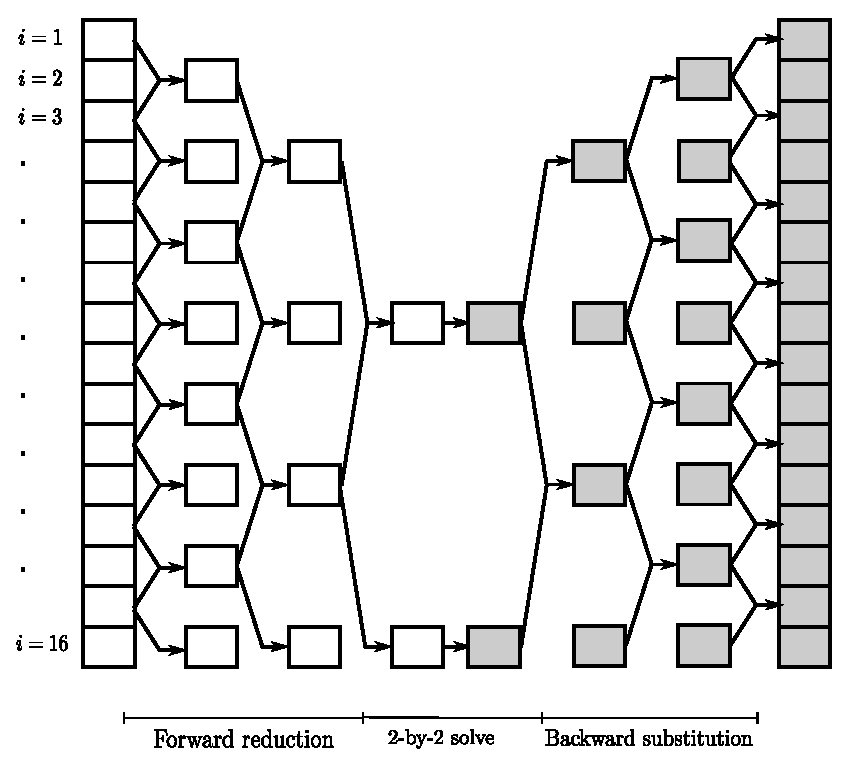
\includegraphics[height=200pt]{img/cyclic-reduction.eps}
\end{center}
\caption{Cyclic reduction.}
\label{fig:cyclic-reduction}
\end{figure}

\subsection{GPU architecture} \label{subsec:gpu-architecture}

Writing applications that effectively exploit the GPU
requires an understanding of the underlying architecture.
We provide the pertinent details here
and refer to \cite{GPUcomputingera} for a more complete picture.
Our tests are performed on the NVIDIA Tesla K20 and K40 GPUs,
built on the ``Kepler'' architecture,
an overview of which is available in \cite{Keplerwhitepaper}.

Applications that use the GPU include special
pieces of code that are executed on the GPU,
referred to as \emph{kernels}.
In C, for example, kernels are written as functions,
and are called with (almost) the same conventions.
A kernel is executed in parallel by several lightweight threads,
which are organized into a \emph{grid} of \emph{thread blocks}
(or just \emph{blocks}).
As a requirement, thread blocks must be able to run
independent of each other,
in series or in parallel.

From the hardware perspective, an NVIDIA GPU may be viewed primarily as
a collection of so-called Streaming Microprocessors (SMs).
When a kernel is launched (with a specified number of thread blocks),
each block is assigned to an SM.
Threads within a thread block can execute concurrently on the SM,
and an SM can execute several thread blocks concurrently.
The number of thread blocks that an SM can execute concurrently
is limited by a number of factors,
and maximizing this number is often key to obtaining good performance.

Every thread in every block has access to so-called \emph{global memory},
which can also be accessed by the CPU (or \emph{host}) via the PCI-e bus.
Further,
threads within a thread block have access
to a common, fast, limited \emph{shared memory}.
The contents of shared memory are managed by the kernel code,
and shared memory is often viewed as an explicitly controlled cache.
Each thread also has private \emph{local memory},
and access to extremely fast registers.
Unlike CPUs, the GPU has a large number of registers---a
thread executing a kernel will
typically attempt to store the variables defined in registers,
before spilling over to local memory, which is much slower.

Thread access to global memory is slow,
and is especially inefficient when
successive threads in a block
access locations that are far apart in memory---known
as \emph{uncoalesced} memory access.
Shared memory access can be expected to be
much faster than global memory---however,
the amount of shared memory per SM is limited
(48 KiB for current GPUs).
The amount of shared memory actually used by each block
can thus limit the number of blocks that
concurrently run on each SM---known as the \emph{occupancy}.
The number of registers per SM is also limited,
and the use of registers can similarly affect occupancy.
Finally, memory transfers between the CPU (host) and GPU (device)
are extremely expensive, limited by the bandwidth of the PCI-e bus.

\subsection{Cyclic reduction implementation on GPU}

\begin{figure}
\begin{center}
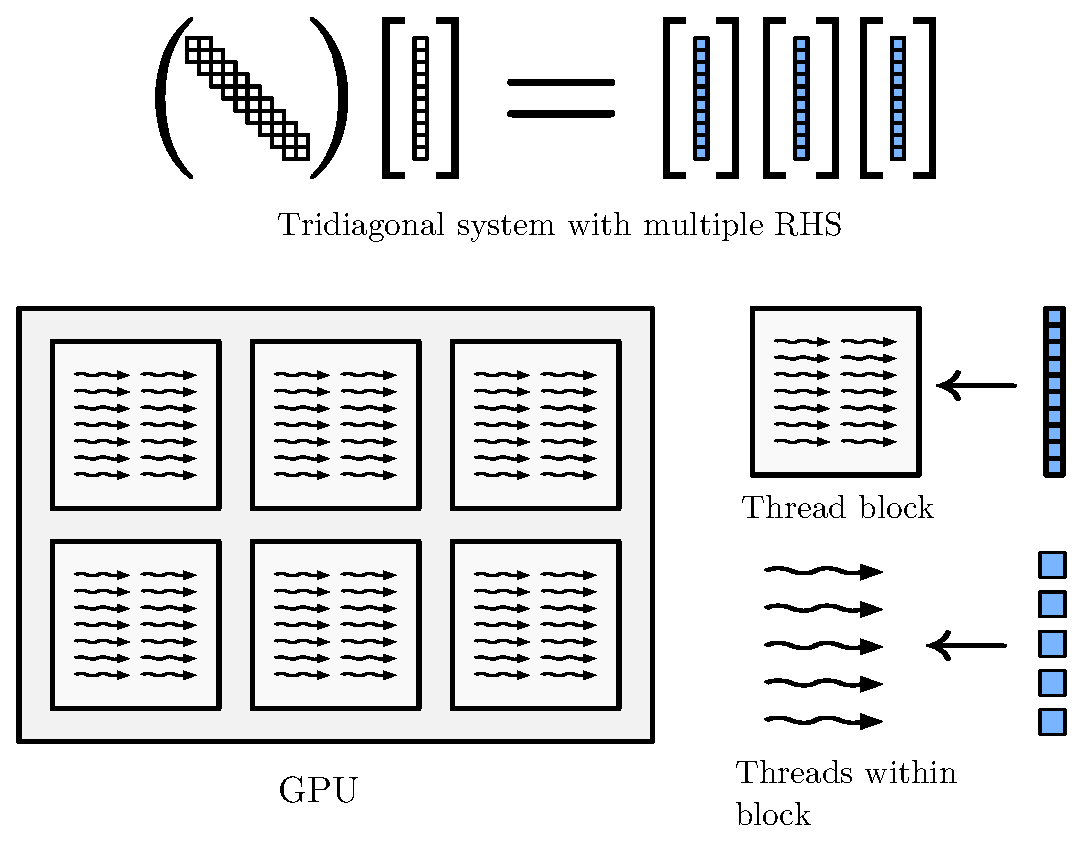
\includegraphics[height=200pt]{img/gpu-mapping.eps}
\end{center}
\caption{Mapping work to blocks and threads:
systems are mapped to blocks and
indices are mapped to individual threads.}
\label{fig:gpu-mapping}
\end{figure}

As described in Section \ref{subsec:gpu-architecture},
GPU instructions are executed concurrently
by several threads and
threads are organized into thread blocks.
In most GPU implementations of cyclic reduction,
blocks are assigned to tridiagonal systems
(when solving multiple systems),
and threads within a block 
are assigned to equations, or \emph{indices}
(Fig. \ref{fig:gpu-mapping}).
During the forward reduction phase,
the threads assigned to each even index $i$
compute the coefficients
$a_i^\prime$, $b_i^\prime$ and $c_i^\prime$.
In practice, the coefficients are updated \emph{in-place}.
Figure \ref{fig:forward-reduction-step} shows the updates
to the coefficient array $\bm{b}$ in the first forward reduction step).

In each step of forward reduction,
a thread accesses values from the coefficient arrays
$\bm{a}$, $\bm{b}$ and $\bm{c}$ in a \emph{strided} fashion.
At every subsequent step,
this stride is doubled, while the number of active threads is halved.
In the backward substitution phase,
the strides are halved at each step,
while the number of active threads is doubled.
The long-strided memory accesses towards the end
of the forward reduction
and the beginning of backward substitution
motivates the use of shared memory---strided global memory access is,
in general, associated with performance penalties.
But the limited amount of shared memory places restrictions
on the size of tridiagonal systems that can be solved.
Further,
the memory access pattern in
cyclic reduction leads to \emph{bank conflicts}
\cite{Zhang2010FTS}.

Much work has been done on optimizing cyclic reduction performance
on GPUs.
Zhang et al. \cite{Zhang2010FTS} propose a
\emph{hybrid} solver
that uses both cyclic reduction and parallel cyclic reduction
to reduce bank conflicts.
G{\"o}ddeke et al. \cite{GoSt11CR}
use a method of separately storing
the even and odd indexed equations
to arrive at a bank-conflict free solver
at the cost of additional shared memory usage.
Shared memory usage is also associated with
lowered GPU occupancy (Section \ref{subsec:gpu-architecture}).
Davidson et al. \cite{davidson2011register}
describe the method of
\emph{register packing}---performing more computations
on \emph{registers}, rather than shared memory---as
a means to reduce shared memory usage in cyclic reduction.
Esfahanian et al., \cite{esfahanian2014efficient}
avoid shared memory (and associated bank conflicts entirely)
using a data rearrangement scheme to improve global memory access.
Our approach takes a different route,
and is focused on \emph{near-Toeplitz} systems---exploiting
the relatively simple matrix structure
to reduce the number of computations and memory accesses
performed by each thread
at every cyclic reduction step.

\begin{figure}
\begin{center}
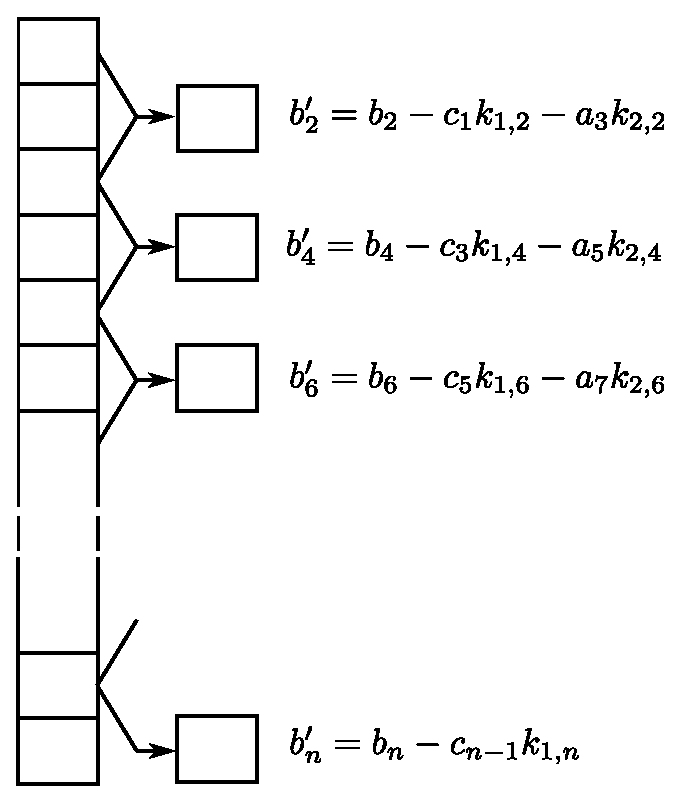
\includegraphics[height=150pt]{img/forward-reduction-step.eps}
\end{center}
\caption{Updating $\bm{b}$ in the first forward reduction step.}
\label{fig:forward-reduction-step}
\end{figure}

%----------------------------------------------------------------------%
\section{Proposed algorithm} \label{sec:proposed-algorithm}
%----------------------------------------------------------------------%

The method is based on precomputing elements 
appearing in the forward reduction phase
so that they can be reused for multiple right hand sides.
While this can be done for general tridiagonal systems,
the applicability to \emph{near-Toeplitz} tridiagonal systems is
of particular interest due to the lower storage costs.
In Fig. \ref{fig:forward-reduction-step},
we list the updates to
$b_i$, for $i=2, 4, 6 ... n$
during the first forward reduction step
for a general tridiagonal matrix.
Similar equations can be written describing
the updates to $a_i$ and  $c_i$.

When the matrix $A$ is \emph{near-Toeplitz} tridiagonal,
if we substitute in the Eqs.
Eqs. (\ref{eqn:forward-reduction-1}) -
(\ref{eqn:forward-reduction-3}):

\begin{itemize}
\item [] $a_2 = a_3 = a_4 = \hdots \equiv a_0$
\item [] $b_2 = b_3 = b_4 = \hdots \equiv b_0$
\item [] $c_2 = c_3 = c_4 = \hdots \equiv c_0$
\end{itemize}
%
we observe that the resulting coefficients
$a_i^\prime$, $b_i^\prime$ and $c_i^\prime$
correspond to the coefficients of a tridiagonal matrix with
exactly the \emph{near-Toeplitz} structure of $A$.
This form-preserving property of cyclic reduction
has been reported for block Toeplitz tridiagonal systems
by Bini et al \cite{bini}.

At each reduction step,
for every index $i$,
the coefficients $a_i^\prime$, $b_i^\prime$, $c_i^\prime$
and auxiliary variables $k_1$ and $k_2$
(hereby denoted as $k_{1,i}$ and $k_{2,i}$) are identical,
except for those influenced by the
boundary coefficients of the previous step.
It is possible to \emph{precompute} these values
and store them in separate arrays.
In Fig. \ref{fig:cyclic-reduction-precomputing},
it is seen that the space required for storing each of the
forward reduction coefficients
$a_i^\prime$, $b_i^\prime$, $c_i^\prime$,
$k_{1,i}$ and $k_{2,i}$
for a \emph{near-Toeplitz} tridiagonal matrix
is, at most, $log_2n-2 + 2(log_2n-1)$.

\begin{figure}
\begin{center}
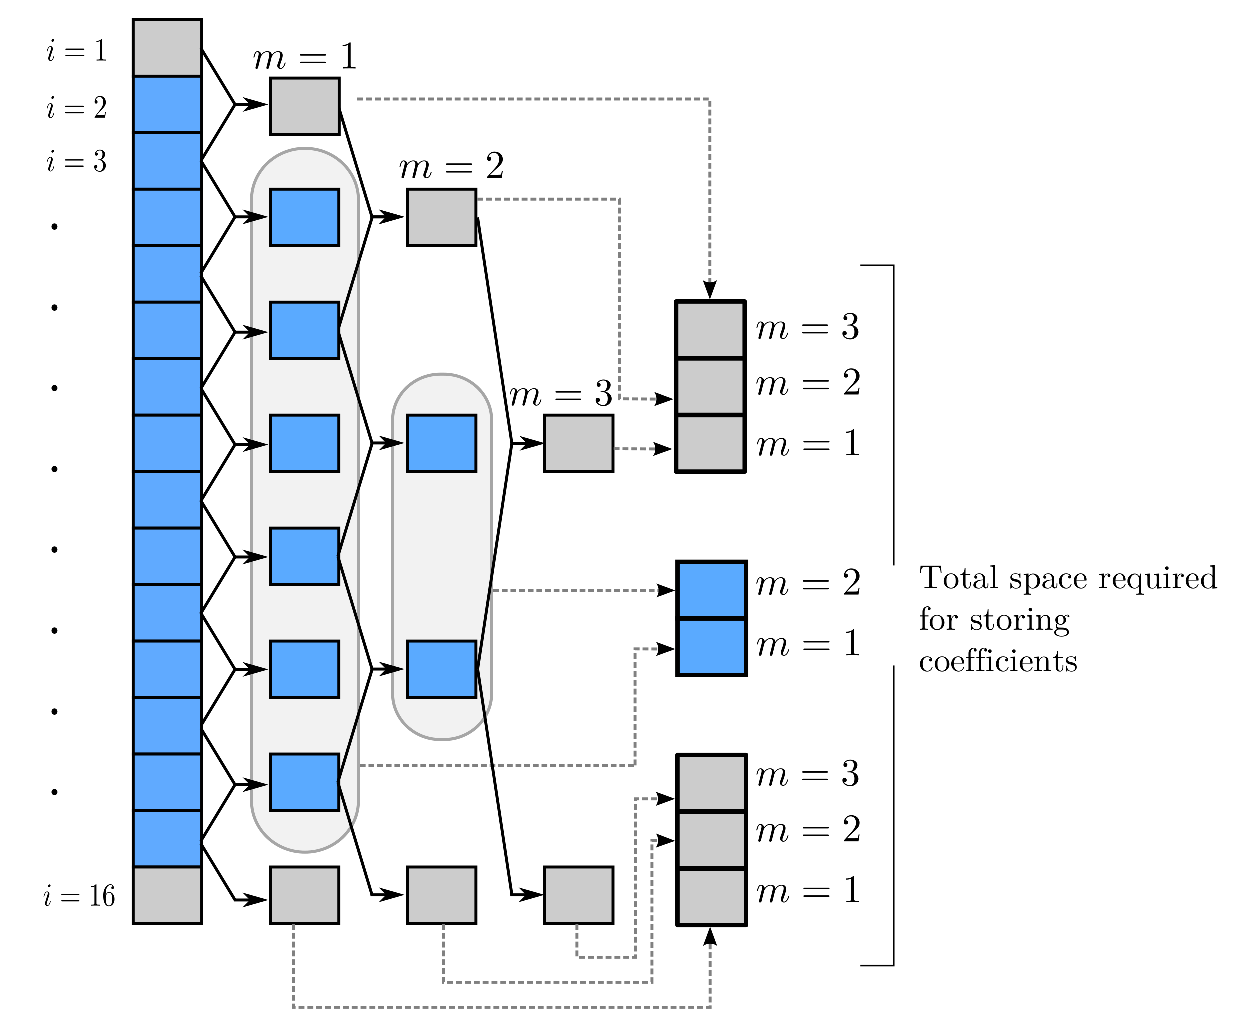
\includegraphics[height=200pt]{img/cyclic-reduction-precomputing.eps}
\end{center}
\caption{Storing forward reduction coefficients
    from each reduction step $m$.}
\label{fig:cyclic-reduction-precomputing}
\end{figure}

By precomputing and storing the forward reduction
coefficients,
the $m^{th}$ forward reduction step is reduced to:

\begin{equation}
d^{\prime}_i = d_i - d_{i-1}k_1^{m}  - d_{i+1}k_2^{m}
\label{eqn:precomputed-forward-reduction-step}
\end{equation}
%
And the $m^{th}$ backward substitution step is:

\begin{equation}
x_i = \frac{d^{\prime}_i - a^mx_{i-1} - \
    c^{m}x_{i+1}}{b^m}
\label{eqn:precomputed-backward-substitution-step}
\end{equation}
%
where $a^m$, $b^m$, $c^m$, $k_1^m$ and $k_2^m$
are the appropriate values
from the precomputed coefficient arrays.
In practice,
the backward substitution step
can overwrite the right-hand side vector $\bm{d}$
with the solution values.

%----------------------------------------------------------------------%
\section{GPU implementation} \label{sec:gpu-implementation}
%----------------------------------------------------------------------%

In this section, we describe the implementation of a GPU solver
for solving a given \emph{near-Toeplitz} tridiagonal system
for $N_{rhs}$ right hand sides.
Our implementation uses the NVIDIA CUDA platform for writing GPU kernels,
interfaced via the Python library PyCUDA \cite{kloeckner_pycuda_2012}.
We develop two approaches based on the common idea
of precomputed forward reduction coefficients---one that leverages
the GPU's \emph{shared memory},
and the other working directly with global memory.
The GPU kernels for both implementations are relatively
straightforward and compact,
spanning no more than 100 lines of code.

Following the algorithm described in Section \ref{sec:proposed-algorithm},
the forward reduction coefficients
are first computed and loaded into global memory.
The right hand sides are stored in a single
contiguous region in global memory.
In both approaches,
we map each of the $N_{rhs}$ tridiagonal systems
to a thread block,
and equations or \emph{indices} of a system
to individual threads within a block
(Fig. \ref{fig:gpu-mapping}).

\begin{figure}
\begin{center}
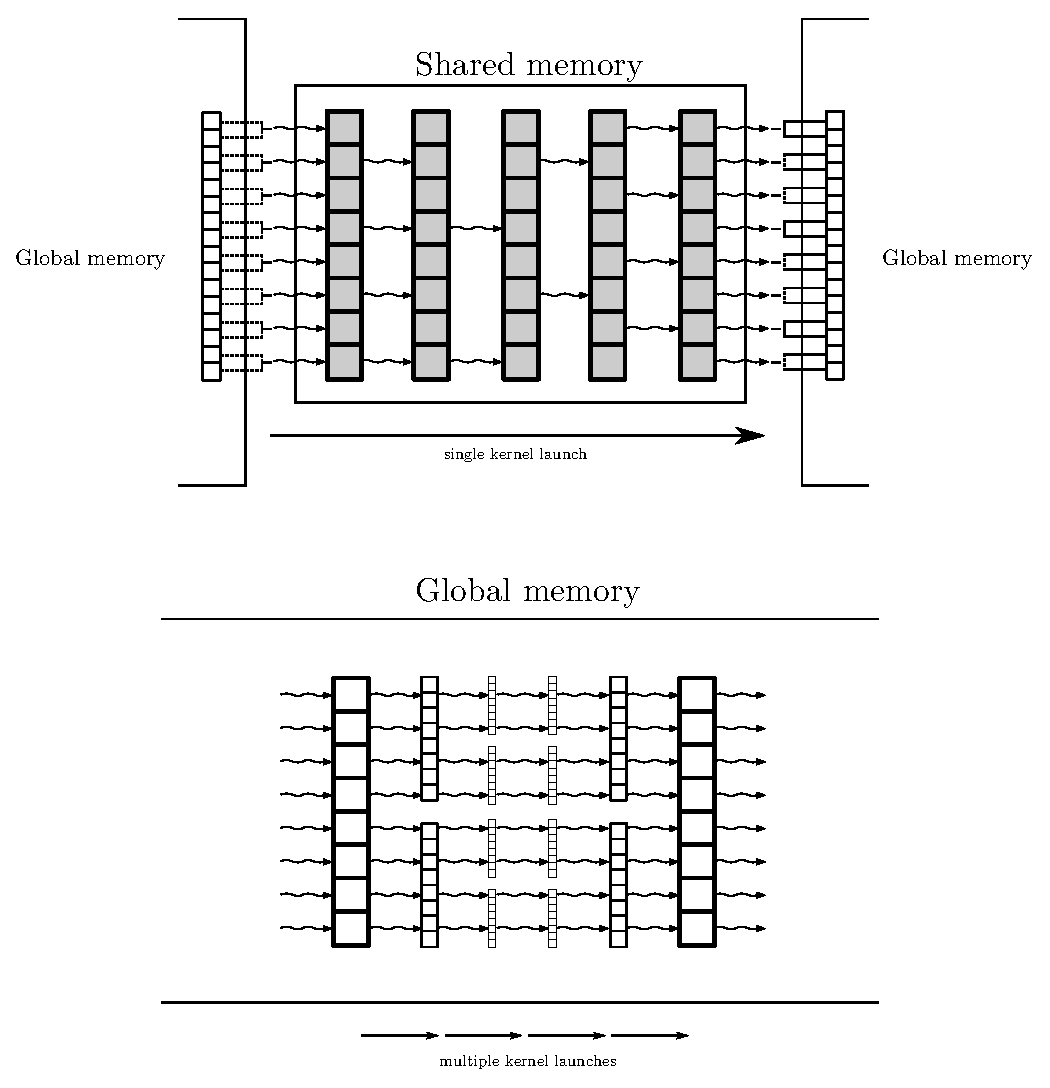
\includegraphics[width=400pt]{img/global-and-shared.eps}
\end{center}
\caption{Thread activity in shared memory (top) and global memory (bottom) implementations.}
\label{fig:global-and-shared}
\end{figure}

\subsubsection*{Global memory}

This implementation works entirely on the GPU's global memory,
Here, we define two kernels - one for the forward reduction step,
and the other for the backward substitution step.
Each kernel is called $log_2(n)-1$ times.
An extra call to the
forward reduction kernel performs
the two-by-two solve.
At each step,
the size of the thread blocks is determined by the \emph{stride}
between elements accessed at that step.
For the forward reduction phase,
we use $n/2$ threads per block for the first step,
$n/4$ threads for the second step, and so on.
The pattern is reversed for the backward substitution phase,
beginning with 2 threads per block for the first step.
Although this ensures that there are no inactive threads
at any stage,
the occupancy of the GPU is still very low
during the end of forward reduction
and the end of backward substitution.

The precomputed coefficient arrays and right hand
are accessed by the kernels from global memory.
The kernel suffers from
strided memory access for the right-hand side,
but the precomputed coefficient values are accessed
without major coalescing problems.
Further, by precomputing the forward reduction coefficients,
we greatly reduce the number of computations
(and thus the number of uncoalesced memory accesses).

\subsubsection*{Shared memory}

In the shared memory approach (Fig. \ref{fig:global-and-shared}),
we launch a single kernel to perform the entire
cyclic reduction solve.
The kernel is launched with $n/2$ threads per block.
Each thread block is allocated a block of shared memory of size $n/2$.
Each thread of a block performs the first reduction step
[Eq. (\ref{eqn:precomputed-forward-reduction-step})]
by accessing the required values
$d_i$, $d_{i-1}$ and $d_{i+1}$ from global memory,
storing the result in shared memory.
In subsequent reduction steps,
$d_i$, $d_{i-1}$ and $d_{i+1}$
are accessed from shared memory,
avoiding the uncoalesced global memory accesses
seen in the global memory implementation.
In each back substitution step,
threads overwrite the existing values in shared memory
with the values of the solution.
In the final step,
shared memory is filled completely
with the even-indexed solution values.
Each thread then computes an odd-indexed solution value,
storing it directly in global memory
and copies the even-indexed solution value
from shared memory to global memory.
The entire solution is done in a single kernel launch
to hide the latency of
memory transfers between global and shared memory.
Explicit synchronization between the threads of a block
is required within the kernel at the end of each step.

The shared memory implementation suffers from two major issues:
first, the number of active threads is halved at each forward reduction step,
(and subsequently doubled at each backward reduction step).
Synchronization between threads of a block is necessary at each step.
Thus, a significant portion of the kernel execution time is
spent by idle threads waiting for active threads to complete execution.
Secondly, the strided access to the
right-hand side values leads to \emph{bank-conflicts}.
However, the number of bank conflicts is significantly smaller
than in cyclic reduction implementations for general tridiagonal systems,
due the reduced number of computations performed.

%----------------------------------------------------------------------%
\section{Results} \label{sec:results-single-gpu}
%----------------------------------------------------------------------%

\begin{figure}
\begin{center}
\includegraphics[width=1.0\linewidth]{fig/global-vs-shared-2d.eps}
\caption{Comparison of global memory and shared
    memory implementations of NEATO (2D problems).}
\label{fig:global-vs-shared-2d}
\end{center}
\end{figure}

\begin{figure}
\begin{center}
\includegraphics[width=1.0\linewidth]{fig/global-vs-shared-3d.eps}
\caption{Comparison of global memory and shared memory
    implementations of NEATO (3D problems).}
\label{fig:global-vs-shared-3d}
\end{center}
\end{figure}

In this section we present a performance overview
of our \emph{near-Toeplitz} tridiagonal solver (NEATO):
against a multi-threaded Intel MKL solver and
the CUSPARSE GPU solver
(\texttt{dgtsv} and \texttt{dgtsvStridedBatch} respectively).
The MKL solver is based on Gaussian Elimination with partial pivoting,
Boundary conditions may prevent
the matrix from being symmetric and/or diagonally dominant,
precluding the use of more specialized tridiagonal solvers.
and the CUSPARSE solver uses a combination of
Cyclic Reduction and Parallel Cyclic Reduction.
Both solvers are optimized for the underlying architectures.

The CPU code is compiled with the Intel C compiler (version 15.0),
and run (with OpenMP support) on up to
16 independent cores of the the same shared-memory node
(one thread per core).
The CPU is an
Intel Xeon Processor E5-2670 v2 (2.50 GHz, 25 MB Smart Cache).
GPU code is compiled with the CUDA toolkit (version 6.5.14),
and run on the
NVIDIA Tesla K20 Accelerator.
When measuring GPU performance (both CUSPARSE and NEATO),
we do \emph{not} include the cost
of data transfer between the CPU and GPU.
\texttt{-O2} level compiler optimizations are enabled for both
CPU and GPU code;
no further optimization options are enabled in either case.
Of course, we use double precision for all solvers.
The timings reported are
kernel \emph{execution} times, i.e.,
the time for all kernel(s) to execute completely
before returning the program control to the CPU.
All timings are averaged over 100 tridiagonal solves.

\subsection{NEATO: global memory v/s shared memory performance}

\begin{figure}
\begin{center}
\includegraphics[width=300pt]{fig/bench-2d.eps}
\caption{Relative solver performance for 2-D problems. Relative time defined as:}
\text{Time taken by solver}/\text{Time taken by NEATO solver}
\label{fig:bench-2d}
\end{center}
\end{figure}

\begin{figure}
\begin{center}
\includegraphics[width=300pt]{fig/bench-3d.eps}
\caption{Relative solver performance for 3-D problems. Relative time defined as:}
$\text{Time taken by solver}/\text{Time taken by NEATO solver}$
\label{fig:bench-3d}
\end{center}
\end{figure}

In Figs. \ref{fig:global-vs-shared-2d} and \ref{fig:global-vs-shared-3d},
we report the performance of the two solvers for the case
$N_{rhs} = n$ and $N_{rhs} = n^2$.
These cases correspond to tridiagonal systems
arising in 2-D and 3-D problems respectively.
We note that the shared memory implementation
offers better performance in nearly all cases.
However, the relative speedup from using
shared memory diminishes with increasing problem size.
For larger problem sizes,
the synchronization costs associated with inactive threads
leads to poor shared memory performance.

\subsection{Comparison of NEATO with Intel MKL and CUSPARSE solvers}

In Fig. \ref{fig:bench-2d} and \ref{fig:bench-3d},
we provide the relative performance of
Intel MKL and CUSPARSE solvers and compare against
the NEATO shared memory implementation.
The relative performance for
each problem size is obtained by
normalizing the solver timings
by the timing for the fastest solver for that problem size.
Table \ref{table:bench} shows the timings of the various
solvers to solve different problem sizes.

\begin{sidewaystable}[]
\scriptsize
\centering
\caption{Performance of Intel MKL, CUSPARSE and NEATO solvers.}
\label{table:bench}
% Please add the following required packages to your document preamble:
% \usepackage{multirow}
\begin{tabular}{|l|l|l|l|l|l|l|}
\hline
\multirow{2}{*}              & \multirow{2}{*}{}        & \multicolumn{5}{c|}{Time to solve (ms)}                             \\ \cline{3-7}
\centering System size       & Number of systems        & MKL 1 core    & MKL 8  cores & CUSPARSE & NEATO (global) & NEATO (shared) \\ \hline
32                           & 32                       & 0.045         & 0.042         & 0.273    & 0.201          & 0.024          \\ \hline
64                           & 64                       & 0.048         & 0.048        & 0.271    & 0.247          & 0.025          \\ \hline
128                          & 128                      & 0.089         & 0.084        & 0.271    & 0.284          & 0.032          \\ \hline
256                          & 256                      & 0.263         & 0.107        & 0.305    & 0.326          & 0.066          \\ \hline
512                          & 512                      & 0.959         & 0.299        & 0.629    & 0.403          & 0.272          \\ \hline
1024                         & 1024                     & 3.775         & 1.023        & 1.939    & 1.375          & 1.252          \\ \hline
2048                         & 2048                     & 16.272        & 4.823        & 7.607    & 5.811          & 10.407         \\ \hline
32                           & 1024                     & 0.152         & 0.094        & 0.31     & 0.207          & 0.092          \\ \hline
64                           & 4096                     & 0.879         & 0.306        & 0.556    & 0.751          & 0.409          \\ \hline
128                          & 16384                    & 7.052         & 2.553        & 3.128    & 3.669          & 2.225          \\ \hline
256                          & 65536                    & 63.858        & 18.792       & 28.495   & 21.148         & 12.565         \\ \hline
512                          & 262144                   & 515.792       & 196.748      &          & 145.34         & 125.311        \\ \hline 
\end{tabular}

\end{sidewaystable}

%----------------------------------------------------------------------
\section{Application: compact finite difference on multiple GPUs}
\label{sec-compact-finite-differences}
%----------------------------------------------------------------------

\begin{figure}
\begin{center}
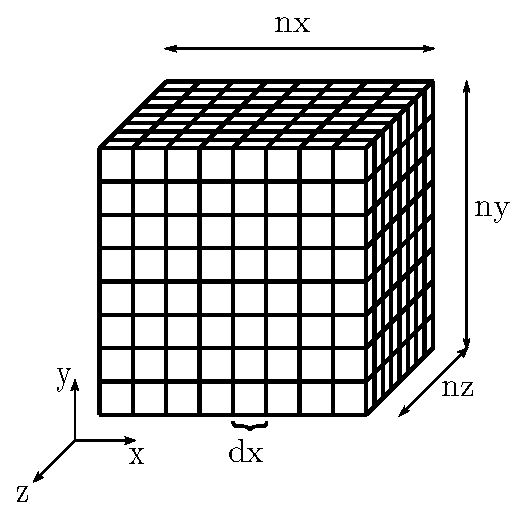
\includegraphics[height=150pt]{img/computational-domain.eps}
\caption{Computational domain in 3-D.}
\label{fig:computational-domain}
\end{center}
\end{figure}

In this section, we present performance details
for evaluating derivatives of a function $f(x, y, z)$
using a compact finite difference scheme.
The numerical algorithm and computational domain are
discussed below:

\subsection{Numerical algorithm}

In a uniformly spaced one-dimensional grid with spacing $dx$,
if $f_i$ represents the value of
the function evaluated at the $i$th node,
the first derivative $f^{\prime}_i$ can be approximated from
a relation of the form:

\begin{equation}
\begin{split}
    \beta(f^{\prime}_{i-2} + f^{\prime}_{i+2}) + \
    \alpha(f^{\prime}_{i-1} + f^{\prime}_{i+1}) + \
        f^{\prime}_i
    = 
    a\frac{f_{i+1} - f_{i-1}}{dx} + \
    b\frac{f_{i+2} - f_{i-2}}{dx} + \\
    c\frac{f_{i+3} - f_{i-3}}{dx} + \
    \hdots
\end{split}
\label{eqn:general-compact}
\end{equation}

For the particular scheme used, $\beta=0$, $\alpha = 1/4$,
$a = 3/4$, and $b = c = \hdots = 0$.
It is easily noted that this leads to a tridiagonal system of equations,
along with a 3-point stencil to evaluate the RHS.
Further, the left boundary can be treated using the following implicit equation:

\begin{equation}
    f^{\prime}_1 + 2f^{\prime}_2 = \frac{-5f_1 + 4f_2 + f_3}{dx}
\end{equation}
%
The right boundary ($f^{\prime}_{n}$) is treated by utilizing
the negative complex-conjugate of the Fourier image of the stencil
at $f^{\prime}_1$:

\begin{equation}
    f^{\prime}_{n} + 2f^{\prime}_{n-1}
    =
    \frac{5f_{n} - 4f_{n-2} -  f_{n-1}}{dx}
\end{equation}
%
This boundary treatment maintains the tridiagonal identity
of the system to be solved, which then has the form:

\begin{equation} \label{eqn:compact-tridiagonal-system}
 \begin{bmatrix}
     1&2\\
     1/4&1&1/4\\
     &1/4&1&1/4\\
     &&1/4&1&1/4\\
     &&&1/4&1&1/4\\
     &&&&&\ddots\\
     &&&&&&\ddots\\
     &&&&&&&\ddots\\
     &&&&&&&2&1
  \end{bmatrix}
  \begin{bmatrix}
      f^{\prime}_1 \\
      f^{\prime}_2 \\
      f^{\prime}_3 \\
      \vdots \\
      \vdots \\
      \vdots \\
      \vdots \\
      f^{\prime}_{n-1} \\
      f^{\prime}_n
   \end{bmatrix}
 =
 \begin{bmatrix}
     \frac{-5f_1 + 4f_2 + f_3}{2}\\
     \frac{3(f_{3} - f_{1})}{4}\\
     \frac{3(f_{4} - f_{2})}{4}\\
     \vdots\\
     \vdots\\
     \vdots\\
     \vdots\\
     \frac{3(f_{n} - f_{n-2})}{4}\\
     \frac{5f_{n} - 4f_{n-1} - f_{n-2}}{2}
  \end{bmatrix}
\end{equation}

\subsection{Computational domain and problem distribution}

The computational domain we consider
(Fig. \ref{fig:computational-domain})
is a structured grid comprised of
$nx \times ny \times nz$ grid points.
While evaluating the derivative in, say, the x-direction,
the computational domain is thought of as
a collection of \emph{grid lines}---each consisting of
$nx$ grid points---oriented in the x-direction.
For each grid line,
we may assemble a tridiagonal system of size $nx$, as in
Eq. (\ref{eqn:compact-tridiagonal-system}).
Solving for the all derivatives in the $x$ direction then involves
solving this tridiagonal system for $ny \times nz$ right hand sides.
Some work has been done on the solution of these
tridiagonal systems using GPUs---Tutkun et al.
\cite{tutkun2012gpu} compute the inverse of the coefficient matrix,
and use the GPU to multiply the inverse with the right-hand sides.
Wei et al. \cite{wei2013parallelizing}
use the parallel cyclic reduction (PCR) algorithm
to solve similar systems appearing in
the 2-D ADI problem.
More recently, Esfahanian et al. \cite{esfahanian2014efficient}
use a variant of cyclic reduction with
data rearrangements kernels for better global memory access patterns.
Our approach uses the NEATO solver described above
to solve for the right hand sides at each grid line,
which takes advantage of the known structure
of the coefficient matrix arising
in the compact finite difference scheme.

When the problem is too large to fit in a single GPU,
it is necessary to \emph{partition} the domain
among multiple \emph{processes} (GPUs).
In this case, each GPU works on a \emph{chunk}, or \emph{subdomain}.
For evaluating compact finite differences along a given direction,
we need only consider the solution strategy for
one line of subdomains.
The other lines may be solved independently and concurrently
in exactly the same manner.

\begin{figure}
\begin{center}
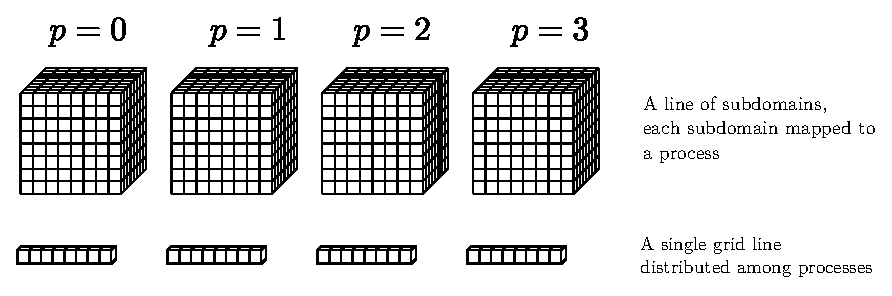
\includegraphics[width=350pt]{img/subdomains-grid-lines.eps}
\caption{A line of subdomains and a single grid line composed of ``local'' grid lines.
    Each subdomain is mapped to a single GPU, or \emph{process},
    and each process is identified by its ``rank''.}
\label{fig:subdomains-grid-lines}
\end{center}
\end{figure}

Figure \ref{fig:subdomains-grid-lines}
shows a line of subdomains
(each of which is mapped to a single process),
and a single grid line
broken into ``local'' grid lines.
For each line of subdomains,
the evaluation of the derivative requires the solution
of Eq. (\ref{eqn:compact-tridiagonal-system})
for each grid line.
The primary difference from the single GPU case is that
the tridiagonal systems are now \emph{distributed}
among several processes.

\subsection{Solving distributed tridiagonal systems}

We use the algorithm
proposed by Mattor et al. \cite{mattor1995algorithm}
for solving the distributed tridiagonal systems.
For a general tridiagonal system $A\bm{x}=\bm{r}$,
the algorithm begins by partitioning
the matrix and right-hand side among the $P$ processes.
Each process $p$ is then associated with the
following $\emph{subsystems}$

\begin{align}
    & A^p\bm{u}^p = \bm{r_u}^p & \label{eqn:secondary-system-1} \\ 
    & A^p\bm{l}^p = \bm{r_l}^p & \label{eqn:secondary-system-2} \\
    & A^p\bm{x_r}^p = \bm{r}^p & \label{eqn:primary-system} 
\end{align}
%
expanded as:

\begin{align}
& \begin{bmatrix}
b_1^p & c_1^p \\
a_2^p & b_2^p & c_2^p \\
      & a_3^p & b_3^p & c_3^p \\
      &       & a_4^p & b_4^p & c_4^p \\
      &       &       &       &  \ddots & c_{m-1}^p\\
      &       &       &       &     a_{m}^p  & b_{m}^p
\end{bmatrix}
\begin{bmatrix}
x_{r,1}^p \\
x_{r,2}^p \\
x_{r,3}^p \\
x_{r,4}^p \\
\vdots \\
x_{r,m}^p
\end{bmatrix}
=
\begin{bmatrix}
r_1^p \\
r_2^p \\
r_3^p \\
r_4^p \\
\vdots \\
r_m^p
\end{bmatrix} & \label{eqn:primary-system-expanded} 
\end{align}

\begin{align}
& \begin{bmatrix}
b_1^p & c_1^p \\
a_2^p & b_2^p & c_2^p \\
      & a_3^p & b_3^p & c_3^p \\
      &       & a_4^p & b_4^p & c_4^p \\
      &       &       &       &  \ddots & c_{m-1}^p\\
      &       &       &       &     a_{m}^p  & b_{m}^p
\end{bmatrix}
\begin{bmatrix}
u_1^p \\
u_2^p \\
u_3^p \\
u_4^p \\
\vdots \\
u_m^p
\end{bmatrix}
=
\begin{bmatrix}
-a_1^p \\
0 \\
0 \\
0 \\
\vdots \\
0
\end{bmatrix} & \label{eqn:secondary-system-1-expanded} 
\end{align}
%
\begin{align}
& \begin{bmatrix}
b_1^p & c_1^p \\
a_2^p & b_2^p & c_2^p \\
      & a_3^p & b_3^p & c_3^p \\
      &       & a_4^p & b_4^p & c_4^p \\
      &       &       &       &  \ddots & c_{m-1}^p\\
      &       &       &       &     a_{m}^p  & b_{m}^p
\end{bmatrix}
\begin{bmatrix}
l_1^p \\
l_2^p \\
l_3^p \\
l_4^p \\
\vdots \\
l_m^p
\end{bmatrix}
=
\begin{bmatrix}
0 \\
0 \\
0 \\
0 \\
\vdots \\
-c_m^p
\end{bmatrix} & \label{eqn:secondary-system-2-expanded}
\end{align}
%
We refer to the subsystem in Eq. (\ref{eqn:primary-system-expanded})
the ``primary'' system, and the subsystems in
Eqs. (\ref{eqn:secondary-system-1-expanded}) and
(\ref{eqn:secondary-system-2-expanded})
the ``secondary'' systems.
Additionally, the following ``reduced'' system is solved:

\begin{align} \label{eqn:reduced-system}
&
\begin{bmatrix}
l^1_m & -1 \\
-1    & u^2_1 & l^2_1 \\
      & u^2_m & l^2_m & -1 \\
      &       & -1    & u^3_1 & l^3_1 \\
      &       &       & u^3_m & l^3_m  & -1 \\
      &       &       &       & \ddots & \ddots & \ddots \\
      &       &       &       &        & -1     & u^P_1
\end{bmatrix}
\begin{bmatrix}
\beta^1 \\
\alpha^2 \\
\beta^2 \\
\alpha^3 \\
\beta^3 \\
\vdots \\
\alpha^P
\end{bmatrix}
=
\begin{bmatrix}
x_{r,m}^1 \\
x_{r,1}^2 \\
x_{r,m}^2 \\
x_{r,1}^3 \\
x_{r,m}^3 \\
\vdots \\
x_{r,1}^P \\
\end{bmatrix}
&
\end{align}
The local part of the solution
is obtained as a linear combination of
the solutions to the primary and secondary systems:

\begin{equation}
    \bm{x}^p = \bm{x}_r^p + \
        \alpha^p \bm{u}^p + \beta^p \bm{l}^p
    \label{eqn:sum-of-systems}
\end{equation}
%
where $\alpha^p$ and $\beta^p$ are obtained
from the solution of the reduced system.

\subsection{GPU implementation}

\begin{figure}
\begin{center}
\includegraphics[trim={0cm 8cm 0cm 8cm},clip,width=500pt]{img/compact-algorithm.pdf}
\centering
\caption{Algorithm for evaluating compact finite differences on multiple GPUs,
(right: CUDA kernels and MPI calls used)}
\label{fig:compact-algorithm}
\end{center}
\end{figure}

We present a specialization of the above algorithm
applied to the distributed tridiagonal systems that
appear in compact finite difference evaluations,
and adapted for GPUs.
Our algorithm is outlined in Fig. \ref{fig:compact-algorithm},
and is described for the case of evaluating derivatives
in the direction along which successive
function values in a subdomain are stored contiguously in memory,
i.e., the ``fastest'' coordinate direction.
Each step of the algorithm must be implemented on the GPU
to avoid data transfer to and from the CPU,
which is prohibitively expensive for large problems.
Thus, we have several kernels to implement the algorithm.
For communication of data between processes,
we use the Message Passing Interface (MPI),
and leverage the NVIDIA GPUDirect Technology
for GPU-GPU communication.
MPI is interfaced via the mpi4py \cite{dalcin2005mpi}
Python library.
The purpose of each CUDA kernel and MPI call used
is described in Table \ref{table:compact-algorithm}.

\begin{table}[]
\centering
\caption{Purpose of kernels and MPI calls in compact finite difference application}
\label{table:compact-algorithm}
\begin{tabular}{|l|p{6cm}|}
\hline
Memcpy3d            & Copy noncontiguous boundary information
                      of the function values
                      to and from contiguous halo arrays \\ \hline
ISend, IRecv        & Perform halo swaps with i-1 and i+1 processes \\ \hline
computeRHSKernel    & Apply pointwise stencil operator to compute
                      RHS at each grid point in the subdomain,
                      using the halo values near the boundaries\\ \hline
NEATO               & Solve the primary tridiagonal systems
                      for the computed right hand sides, giving $x_r$ \\ \hline
copyFacesKernel     & Copy the left and right faces of $x_r$
                      into a single contiguous array \\ \hline
MPI\_Gather         & Gather the data required to assemble
                      the reduced system at rank 0 \\ \hline
reducedSolverKernel & Solve the reduced systems for parameters
                      $\alpha^p$ and $\beta^p$
                      for each grid line \\ \hline
MPI\_Scatter        & Scatter the parameters 
                      $\alpha^p$ and $\beta^p$
                      from rank 0 to all the processes \\ \hline
sumSolutionsKernel  & Sum the primary and secondary solutions
                      to compute the local part of the solution \\ \hline
\end{tabular}
\end{table}

\begin{figure}
\begin{center}
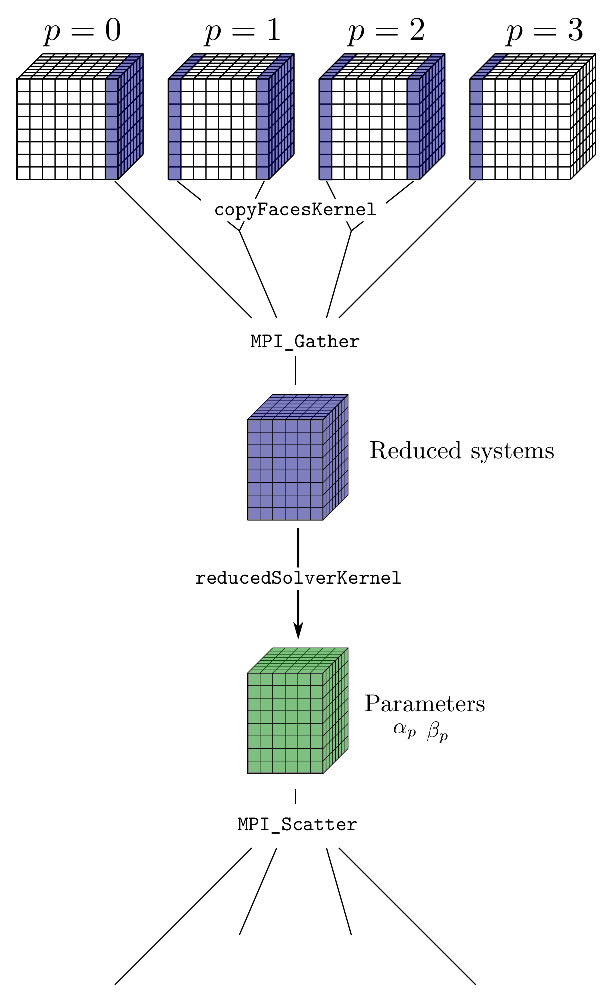
\includegraphics[width=200pt]{img/constructing-reduced-system.eps}
\caption{Construction of the reduced system and scattering of parameters.}
\label{fig:constructing-reduced-system}
\end{center}
\end{figure}

First, we note that
the secondary systems
[Eq. (\ref{eqn:secondary-system-1-expanded}) and
 Eq. (\ref{eqn:secondary-system-2-expanded})]
are dependent only on $\bm{a}$, $\bm{b}$ and $\bm{c}$,
the tridiagonal coefficients of the global tridiagonal system.
\hl{These are the same for all local grid lines,
so they are \emph{precomputed} -
solved \emph{once} for a single local grid line in each subdomain.
This is done on the CPU.}

The primary system [Eq. (\ref{eqn:primary-system-expanded})] must be solved
for each of the local grid lines in a subdomain,
as the right hand sides are different at each of the local grid lines. 
The evaluation of the right hand sides are
pointwise stencil computations,
which require communication of the
function values at the boundaries of the subdomains.
This is achieved using a halo-swapping technique
with dedicated contiguous halo arrays for each subdomain,
as communication of non-contiguous MPI
data types is expensive on the GPU.
The primary system is solved for all the local grid lines
using the NEATO solver.

The set up and solution of the reduced system
requires global communication of the boundary information
from the solutions $\bm{u}^p$, $\bm{l}^p$ and $\bm{x_r}^p$.
The tridiagonal coefficients of the reduced system
are set up easily,
by communicating the boundary elements from
$\bm{u}^p$ and $\bm{l}^p$,
which are the same for every local grid line in each subdomain.

The right hand sides require significantly more communication,
as they are assembled from the boundary elements of $\bm{x_r}^p$,
which are different for each local grid line in each subdomain.
Thus, the boundary ``faces'' of each subdomain need to be communicated.
These faces are first copied into a contiguous array,
and these arrays are gathered at rank 0
to assemble the right-hand sides of the reduced system
(Fig. \ref{fig:constructing-reduced-system}).
This communication strategy has the effect of
producing right hand sides aligned along the
``slowest'' co-ordinate direction, i.e.,
the right hand side values for neighboring grid points
are located far apart in memory.
As the reduced systems are quite small relative to the primary systems,,
we use a convenient, but rather inefficient
\emph{p-Thomas} algorithm to solve the systems,
wherein each GPU thread solves the reduced system
for a single grid line using the Thomas algorithm.
The solution of the reduced systems produces the parameters
$\alpha^p$ and $\beta^p$,
which are scattered back to the respective processes, $p$.

Finally, the summing of the solutions
is a pointwise operation that is easily implemented
on the GPU.
For evaluation of compact finite differences in other
coordinate directions,
a local permutation of the data is performed on the input data
(function values)
before applying the above algorithm,
and again on the output data
(derivative values).

\subsection{Results}

Here, we provide performance results for
evaluating derivatives using the above approach
for large, distributed problems.

The experiments were run on the
Clemson University Palmetto Cluster,
using NVIDIA Tesla K20 and K40 GPUs.
The K40 GPUs were used for the largest problem sizes.
Each compute node on the cluster is equipped with up to 2 GPUs,
and nodes are connected by 56 Gbps Infiniband interconnect.
We use Open MPI 1.8.1 configured with OpenFabrics support.

The timings reported are \emph{wall clock} times
with global synchronization between processes performed 
before and after evaluation of the derivatives.
All timings are averaged over 100 evaluations of the function derivatives
in each coordinate direction.
We make it clear that our reported
problem sizes represent the \emph{actual size of problem data}.
Although it may be considered sufficient to
run tests on a single line of processes
for measuring the compact finite difference solver performance,
we set up and solve the problem for the entire computational domain.
In the context of a larger simulation,
global synchronization between the processes
is typically performed before and after the evaluation of derivatives,
and it is important to consider the related overhead.

Figures \ref{fig:compact-profiling-1024-64}-\ref{fig:compact-profiling-2048-64}
show the time taken by the different steps of
the compact finite difference solver.
We note that for the larger problem size,
the evaluation of the primary systems (using the NEATO solver)
constitutes a larger majority of the total runtime,
which justifies our efforts in optimizing the tridiagonal solver.
For evaluation of the derivatives in the y- and z- directions,
we note that a significant portion of the runtime is dedicated
to performing permutations of the input and output data.
We attribute this to our naive implementation of the
permutation kernels (no shared memory).
Figures \ref{fig:strong-scaling-256}-\ref{fig:weak-scaling-256}
show the strong and weak scaling of the compact finite difference solver
for evaluating derivatives in all three coordinate directions.
We note good scaling for both 2-D and 3-D cases.
The strong scaling for 3-D problems is somewhat better
as the GPU is kept busy for all problem sizes.

\begin{figure}
\begin{center}
\includegraphics[width=300pt]{fig/profiling-1024-64.eps}
\caption{Solving problem sized $1024^3$ on 64 GPUs}
\label{fig:compact-profiling-1024-64}
\end{center}
\end{figure}

\begin{figure}
\begin{center}
\includegraphics[width=300pt]{fig/profiling-2048-64.eps}
\caption{Solving problem sized $2048^3$ on 64 GPUs}
\label{fig:compact-profiling-2048-64}
\end{center}
\end{figure}

\begin{figure}
\begin{center}
\includegraphics[width=300pt]{fig/strong-scaling-256.eps}
\caption{Strong scaling for multi-GPU compact finite difference, problem size: $256^3$.}
\label{fig:strong-scaling-256}
\end{center}
\end{figure}

\begin{figure}
\begin{center}
\includegraphics[width=300pt]{fig/strong-scaling-512.eps}
\caption{Strong scaling for multi-GPU compact finite difference, problem size: $512^3$.}
\label{fig:strong-scaling-512}
\end{center}
\end{figure}

\begin{figure}
\begin{center}
\includegraphics[width=300pt]{fig/weak-scaling-128.eps}
\caption{Weak scaling for multi-GPU compact finite difference, problem size: $128^3$ per process.}
\label{fig:weak-scaling-128}
\end{center}
\end{figure}

\begin{figure}
\begin{center}
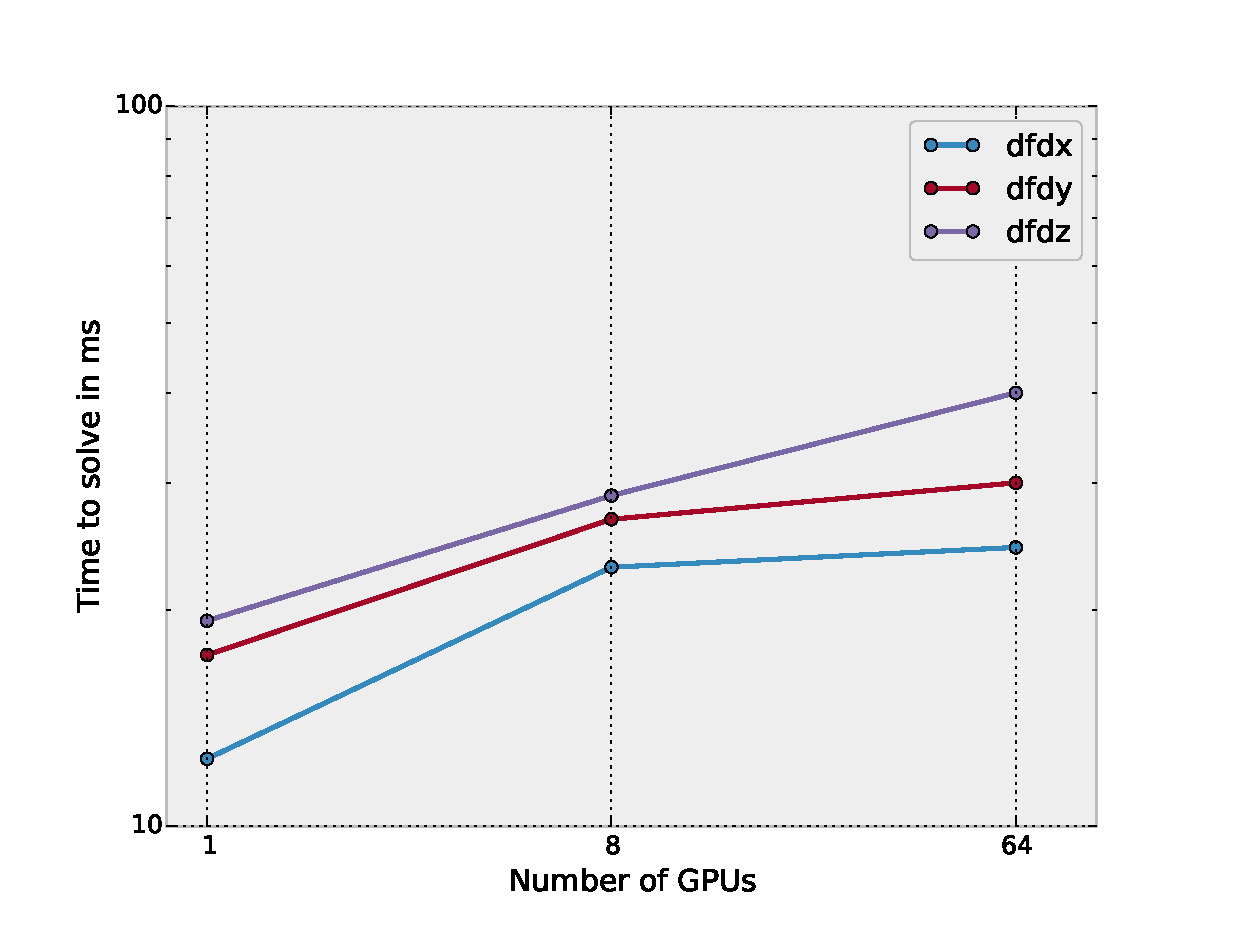
\includegraphics[width=300pt]{fig/weak-scaling-256.eps}
\caption{Weak scaling for multi-GPU compact finite difference, problem size: $256^3$ per process.}
\label{fig:weak-scaling-256}
\end{center}
\end{figure}

\section{Conclusions}

We present a GPU solver for \emph{near-Toeplitz} tridiagonal systems
based on the cyclic reduction algorithm,
that is applicable to several numerical schemes
in computational fluid dynamics.
Our solver gives better performance than
the current multicore Intel MKL and CUSPARSE solvers
Additionally, we describe an implementation of our solver
for GPU clusters,
and provide performance results for a
compact finite difference application,
run on up to 64 GPUs.

\pagebreak
\section*{References}
\bibliography{references}
\bibliographystyle{elsarticle-num}
\end{document}
